%% 《高级图论》课程论文（Codex V3）
%% 版式参照 classPaper/V3 的 CjC 单栏格式，并使用可直接编译的 ctexart 实现
\documentclass[UTF8,a4paper,zihao=5,fontset=fandol]{ctexart}

\newcommand{\CourseName}{高级图论}
\newcommand{\StudentName}{杜浩存}
\newcommand{\Affiliation}{西安交通大学\quad 西安\quad 710049}

\usepackage[left=2.20cm,right=2.20cm,top=2.05cm,bottom=2.10cm,headheight=14pt]{geometry}
\usepackage{amsmath,amssymb,amsfonts,bm,mathtools}
\usepackage{graphicx}
\usepackage{booktabs,multirow,tabularx,array,threeparttable}
\usepackage{caption,subcaption}
\usepackage{enumitem}
\usepackage{float}
\usepackage{microtype}
\usepackage{xcolor}
\usepackage{fancyhdr}
\usepackage{url}
\usepackage{tikz}
\usetikzlibrary{arrows.meta,positioning,calc,fit,backgrounds}
\usepackage[numbers,sort&compress]{natbib}
\usepackage[hidelinks,bookmarksnumbered=true]{hyperref}
\usepackage[nameinlink,noabbrev]{cleveref}

\graphicspath{{figures/}}
\setlength{\parindent}{2em}
\setlength{\parskip}{0pt}
\linespread{1.10}
\setlist{nosep,leftmargin=2em}
\captionsetup{font=small,labelfont=bf,labelsep=quad,skip=5pt}
\renewcommand{\figurename}{图}
\renewcommand{\tablename}{表}
\renewcommand{\refname}{参考文献}
\newcolumntype{Y}{>{\centering\arraybackslash}X}
\newcommand{\Rtwo}{R^2}
\newcommand{\vtrue}{v_c(S)}
\newcommand{\vhat}{\widehat v_c(S)}
\newcommand{\indicator}{\mathbb{I}}
\newcommand{\method}{GSSO}

\ctexset{
  section={
    format=\zihao{4}\bfseries\heiti,
    beforeskip=1.35ex plus .25ex minus .2ex,
    afterskip=.65ex
  },
  subsection={
    format=\zihao{5}\bfseries\heiti,
    beforeskip=1.05ex plus .2ex minus .15ex,
    afterskip=.4ex
  },
  subsubsection={
    format=\zihao{5}\bfseries\heiti,
    beforeskip=.8ex,
    afterskip=.25ex
  }
}

\pagestyle{fancy}
\fancyhf{}
\fancyhead[L]{\zihao{-5}\StudentName}
\fancyhead[R]{\zihao{-5}图结构集合敏感度与协同推断}
\fancyfoot[C]{\zihao{-5}\thepage}
\renewcommand{\headrulewidth}{0.4pt}
\renewcommand{\footrulewidth}{0pt}

\hypersetup{
  pdftitle={面向任意字段集合的图结构推断敏感度评估与协同泄露发现},
  pdfauthor={\StudentName},
  pdfsubject={高级图论课程论文},
  pdfkeywords={推断图, 集合函数, 图神经网络, 数据敏感度, 协同推断}
}

\begin{document}
\thispagestyle{empty}
\vspace*{-9mm}
\noindent{\zihao{-5}\StudentName\hfill 《\CourseName》课程论文\hfill 2026 年 7 月}\par
\vspace{1mm}
\noindent\rule{\textwidth}{0.8pt}

\begin{center}
\vspace{7mm}
{\zihao{2}\heiti 面向任意字段集合的图结构推断敏感度评估\\[1mm]
与协同泄露发现\par}
\vspace{4mm}
{\zihao{4}\fangsong \StudentName\par}
\vspace{2mm}
{\zihao{5}\songti（\Affiliation）\par}
\end{center}

\vspace{4mm}
{\zihao{5}\setlength{\baselineskip}{16pt}\selectfont
\noindent{\heiti 摘\quad 要\quad}
传统数据敏感度评估通常为单个字段给出独立分数，但在电力数据中，多个单独风险较低的字段可能通过物理恒等式或统计耦合共同推断出机密字段，因此敏感度本质上是定义在字段幂集上的集合函数。本文提出一种面向任意字段集合的图结构推断敏感度框架。首先，将可见字段与机密字段表示为带权推断图，并将集合敏感度定义为攻击者仅观察集合 $S$ 时能够达到的截断决定系数 $v_c(S)$；其次，分别使用专用 DNN/GCN 攻击者刻画经验推断上限，使用随机掩码通用 Oracle 摊销指数级子集空间的扫描成本，并以少步微调和逐集合重训练完成候选认证；最后，从 $v_c(S)$ 中导出二阶协同边与三阶协同超边，使“任意集合敏感度”成为主问题，而协同推断成为集合函数上的结构化结果。在 8760 条 PJM RTO 小时级记录、44 个可见字段和 12 个机密字段上，50 个宽尺寸随机集合的最优经验推断能力随集合规模由 $0.2311$ 增至 $0.8647$。专用 GCN 在 5--8 和 9--16 字段区间分别比 DNN 高 $0.0235$ 和 $0.0130$，总体平均高 $0.0072$。采用 MLP Oracle 微调 500 步后，二阶协同排序相对重训真值的 Spearman 相关系数达到 $0.9597$，top-20 重合率为 $0.95$，单集合耗时约 $1.01$ s。重训认证进一步发现 $0.765$ 的二阶增量协同与 $0.455$ 的不可约三阶协同。结果说明，以推断图、集合函数和协同图联合描述数据风险，能够发现单字段排序无法表达的组合泄露路径。\par}

\vspace{2mm}
\noindent{\zihao{5}\heiti 关键词\quad}
{\zihao{5}推断图；集合函数；图神经网络；数据敏感度；协同推断；高阶超图}

\begin{center}
\vspace{6mm}
{\zihao{3}\heiti Graph-Structured Inference Sensitivity for Arbitrary Field Sets\\[-0.5mm]
and Synergistic Leakage Discovery\par}
\vspace{3mm}
{\zihao{5}DU Hao-Cun\par}
\vspace{1mm}
{\zihao{-5}(Xi'an Jiaotong University, Xi'an 710049, China)\par}
\end{center}

\vspace{3mm}
{\zihao{5}\setlength{\baselineskip}{17pt}\selectfont
\noindent\textbf{Abstract}\quad
Field-wise sensitivity scores cannot describe a key risk in power-system data: several fields that are weak individually may jointly reveal a confidential target through physical identities or statistical dependence. We formulate sensitivity as a set function over the power set of observable fields and propose a graph-structured sensitivity-oracle framework. Observable and confidential fields form a weighted inference graph. Dedicated DNN and GCN attackers estimate the empirical attack upper bound, while a random-mask universal oracle scans arbitrary subsets at low marginal cost; fine-tuning and subset-specific retraining are then used for certification. Experiments on 8,760 hourly PJM RTO records with 44 observable and 12 confidential fields show that the empirical attack score increases from 0.2311 to 0.8647 as the subset-size band grows. A dedicated GCN exceeds a DNN by 0.0235 and 0.0130 in the 5--8 and 9--16 bands. With 500 fine-tuning steps, the pairwise-synergy ranking reaches a Spearman correlation of 0.9597 and a top-20 overlap of 0.95 against retraining truth at about 1.01 seconds per subset. Certified examples include a pairwise increment of 0.765 for wind generation and wind share inferring total generation, and an irreducible third-order increment of 0.455 for gas generation, gas share, and load forecast inferring net interchange.\par}

\vspace{2mm}
\noindent\textbf{Keywords}\quad graph neural network; set function; data sensitivity; synergistic inference; hypergraph
\vspace{7mm}

\pagestyle{fancy}

\section{引言}

电力系统公开数据通常同时包含负荷、燃料发电量、燃料占比、市场价格、辅助服务和交换功率等字段。即使某个机密字段从未被直接公开，攻击者仍可能利用可见字段之间的物理约束与统计关系进行间接推断。这类风险与传统“数据库是否被入侵”的问题不同：它关注的是在合法获得一组普通字段后，机密字段还剩下多少不可预测性。模型反演与属性推断研究已经表明，非敏感属性和模型输出能够被用于恢复未知敏感属性\citep{fredrikson2015model,mehnaz2022sensitive}；近期面向电力系统的 IGNN 工作进一步把字段间推断关系表示为图，并利用图注意力传播敏感度\citep{hu2026ignn}。

然而，仅为每个字段分配一个独立敏感度仍不充分。以“燃料发电量”和“该燃料发电占比”为例，两者单独可能只提供有限信息，但合并后可通过近似关系
\begin{equation}
  \text{总发电量}\approx
  \frac{\text{某燃料发电量}}{\text{该燃料发电占比}}
\end{equation}
恢复高敏感目标。此时，风险不是任一字段单独携带的，而是由集合形成的。若共有 $n$ 个可见字段，则潜在集合数为 $2^n$；本文数据中 $n=44$，无法为每个集合都从头训练攻击模型。进一步地，若直接在一个只见过完整输入的模型上把缺失字段置零，评估结果可能主要反映分布外失真，而不是“攻击者只拥有集合 $S$”时的真实能力。

本文的核心问题因此不是“哪些字段两两协同”，而是：
\begin{quote}
\centering
\emph{如何构造一个能够查询任意可见字段集合 $S$ 的敏感度 Oracle，并在此基础上可靠发现二阶和更高阶协同推断结构？}
\end{quote}

为回答该问题，本文提出图结构集合敏感度 Oracle 框架（Graph-structured Set Sensitivity Oracle，\method）。该框架以集合敏感度为核心对象，以字段推断图提供关系先验，并以协同图和高阶超图表示由集合函数导出的组合泄露结构。主要贡献如下。

\begin{enumerate}
  \item \textbf{集合函数形式化。} 将每个可见字段视为合作博弈中的“参与者”，把机密字段 $c$ 的可推断性写成 $v_c:2^{V_g}\rightarrow[0,1]$，从而统一描述单字段敏感度、任意集合敏感度和协同增量。
  \item \textbf{图结构攻击上限与通用 Oracle 分层。} 用带权推断图上的专用 GCN 和 DNN 共同审计固定集合的经验推断上限；用随机掩码训练的通用 Oracle 低成本扫描指数级空间，再通过微调和重训认证闭合摊销误差。
  \item \textbf{协同图与高阶超边。} 从同一个 $v_c(S)$ 导出保守的二阶协同边和三阶增量超边，并以噪声底决定边是否可信，避免把训练随机波动误写成协同。
  \item \textbf{基于真实项目产物的系统实验。} 在 1437 个评测条目上区分“专用 GCN 攻击者是否更强”和“通用 GNN Oracle 是否更准”，并穷举 946 个字段对、扫描全部 $\binom{44}{3}=13244$ 个三元组，给出可解释的二阶与三阶案例。
\end{enumerate}

\section{问题定义与图论建模}

\subsection{威胁模型与符号}

设数据表由可见字段集合 $V_g=\{1,\dots,n\}$ 和机密字段集合 $V_c=\{1,\dots,q\}$ 构成。攻击者能够获得同分布辅助样本，并观察目标样本在集合 $S\subseteq V_g$ 上的取值 $X_S$，但不能直接观察 $Y_c$。攻击者可训练回归模型 $f_{\theta,S}:X_S\rightarrow Y_c$。本文关注字段关系导致的\emph{总体可推断性}，不声称恢复某一特定用户的训练记录；数据切分和指标都在独立测试集上计算。

表\ref{tab:notation}列出主要符号。集合 $S$ 既可包含一个字段，也可包含任意多个字段。与传统单点打分相比，$S$ 是方法中的第一等对象。

\begin{table}[H]
  \centering
  \caption{主要符号}
  \label{tab:notation}
  \begin{tabularx}{0.94\textwidth}{@{}lX@{}}
    \toprule
    符号 & 含义\\
    \midrule
    $G=(V,E,W)$ & 字段推断图，$V=V_g\cup V_c$，$W$ 为多关系权重\\
    $S\subseteq V_g$ & 攻击者可观察的字段集合\\
    $m_S\in\{0,1\}^{n}$ & 集合 $S$ 的可见性掩码\\
    $v_c(S)$ & 集合 $S$ 对机密字段 $c$ 的理论推断敏感度\\
    $\widehat v_c(S)$ & 通用 Oracle 或有限攻击模型给出的经验估计\\
    $\Delta_c(i,j)$ & 字段 $i,j$ 对目标 $c$ 的二阶增量协同\\
    $\Delta_c^{(3)}(i,j,k)$ & 三元组相对其最好二元子集的三阶增量协同\\
    $\mathcal A$ & 允许的攻击模型族，例如 DNN 与 GCN\\
    \bottomrule
  \end{tabularx}
\end{table}

\subsection{字段推断图}

将全部字段表示为带权有向图
\begin{equation}
  G=(V_g\cup V_c,E,W).
\end{equation}
可见字段之间的边描述冗余与替代关系，可见字段指向机密字段的边描述直接推断通道。对字段 $i,j$，本文计算 Pearson、Spearman、Kendall、归一化互信息和距离相关五种关系度量，经归一化后求平均得到初始权重
\begin{equation}
  \widetilde w_{ij}=\frac{1}{5}\sum_{r=1}^{5}\rho^{(r)}_{ij}.
\end{equation}
随后保留每个节点的 top-$k$ 关系并施加阈值 $\tau$，得到稀疏边集
\begin{equation}
  E=\{(i,j):\widetilde w_{ij}\ge \tau,\ j\in\operatorname{TopK}(i)\}.
\end{equation}
实验取 $k=8,\tau=0.15$，并对可见字段子图进行对称化。该构图方式不把相关性直接等同于泄露，只把它作为消息传递的结构先验；最终敏感度必须由测试集上的攻击效果定义。

\subsection{任意集合敏感度}

对给定机密字段 $c$ 和可见集合 $S$，理论敏感度定义为允许攻击模型族中的最优测试集推断能力：
\begin{equation}
  v_c(S)=\sup_{f\in\mathcal A}
  \left[
  1-\frac{\sum_{t\in\mathcal D_{\mathrm{te}}}
  (y_{t,c}-f(x_{t,S}))^2}
  {\sum_{t\in\mathcal D_{\mathrm{te}}}
  (y_{t,c}-\overline y_c)^2+\epsilon}
  \right]_+,
  \label{eq:setvalue}
\end{equation}
其中 $[z]_+=\max(z,0)$。使用截断 $\Rtwo$ 的原因是：负 $\Rtwo$ 只表示攻击器比均值基线更差，不应被解释为“负敏感度”。多目标总分定义为
\begin{equation}
  v(S)=\frac{1}{q}\sum_{c=1}^{q}v_c(S).
\end{equation}

从图论角度看，原始字段图 $G$ 描述局部关系，而 $v_c$ 定义在布尔格 $2^{V_g}$ 上。理论上，当攻击模型族足够丰富且训练达到最优时，若 $S\subseteq T$，攻击者可以忽略 $T\setminus S$，故应有 $v_c(S)\le v_c(T)$。有限样本、有限优化和随机初始化会造成轻微非单调，因此本文使用多结构上包络、微调和重训认证逼近式\eqref{eq:setvalue}，而不把一次模型前向误认为数学上精确的上确界。

\section{图结构集合敏感度 Oracle}

\subsection{总体框架}

如图\ref{fig:framework}所示，\method 包含三个层次。第一层是字段推断图和固定集合的专用攻击者，用于刻画强攻击能力；第二层是接受集合掩码的通用 Oracle，用一次训练覆盖大量集合；第三层由集合函数生成协同图和高阶超边。计算流程遵循“全空间扫描 $\rightarrow$ 少步微调 $\rightarrow$ 候选重训认证”，把计算预算集中在可能具有强协同的少量集合上。

\begin{figure}[H]
  \centering
  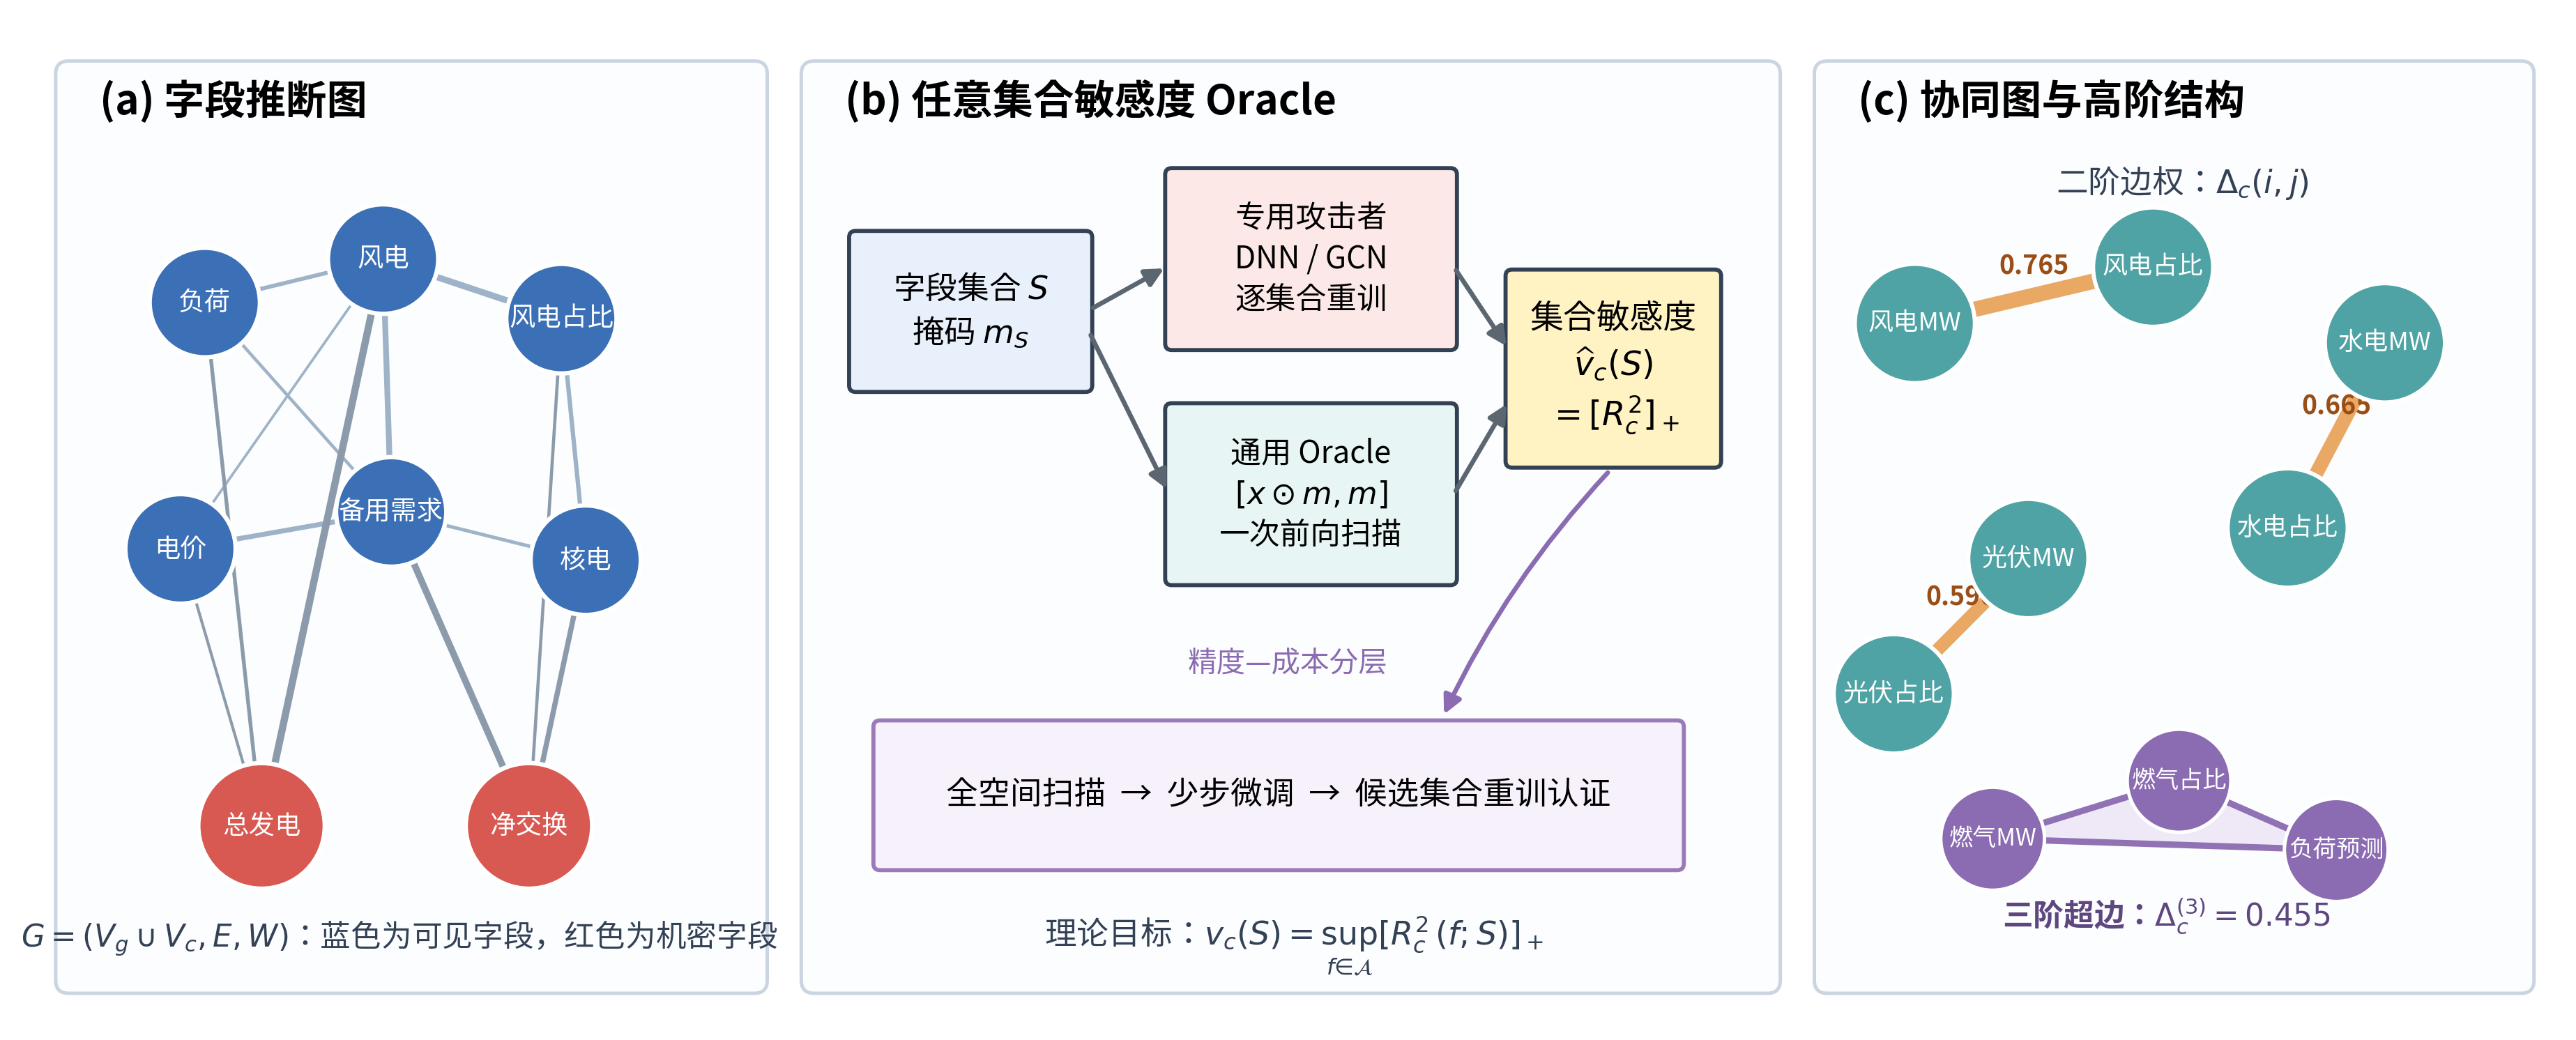
\includegraphics[width=\textwidth]{framework.png}
  \caption{\method 总体框架。核心输出是任意集合的 $v_c(S)$；二阶协同图和三阶超边均由该集合函数导出。}
  \label{fig:framework}
\end{figure}

\subsection{固定集合的专用 DNN/GCN 攻击者}

对每个固定集合 $S$，专用攻击者只在 $X_S$ 上训练。DNN 将可见字段拼接后输入多层感知机；GCN 则在诱导可见子图 $G[S\cup V_c]$ 上共享消息传递参数。第 $\ell$ 层的可见性感知聚合写为
\begin{align}
  \alpha_{ij}^{(\ell)}(S)
  &=
  \frac{\indicator[j\in S]\,
  \exp\left(e_{ij}^{(\ell)}+\lambda\log(w_{ij}+\epsilon)\right)}
  {\sum_{r\in\mathcal N(i)\cap S}
  \exp\left(e_{ir}^{(\ell)}+\lambda\log(w_{ir}+\epsilon)\right)},\\
  h_i^{(\ell+1)}
  &=
  \sigma\left(
  W_{\mathrm{self}}^{(\ell)}h_i^{(\ell)}
  +
  \sum_{j\in\mathcal N(i)\cap S}
  \alpha_{ij}^{(\ell)}(S)W_{\mathrm{msg}}^{(\ell)}h_j^{(\ell)}
  \right).
  \label{eq:visible_gnn}
\end{align}
被遮蔽节点既不提供数值，也不参与 softmax 归一化。因此当某条直接路径不可见时，注意力能够沿仍可见的相关邻居重分配。该机制与 GCN 的局部结构编码\citep{kipf2017gcn}和 GAT 的邻域注意力\citep{velickovic2018gat}一致，但这里的节点是数据字段而不是电网母线。

\begin{figure}[H]
  \centering
  \resizebox{0.99\textwidth}{!}{\begin{tikzpicture}[
  x=1cm,y=1cm,
  font=\zihao{-5},
  flow/.style={-{Stealth[length=2.2mm,width=1.5mm]},line width=0.85pt,draw=black!62},
  panel/.style={rounded corners=2.5pt,draw=black!38,fill=white,line width=0.7pt,align=center},
  stage/.style={font=\zihao{-5}\bfseries\heiti,text=black!78,align=center},
  note/.style={font=\zihao{-5},text=black!62,align=center},
  visible/.style={rounded corners=1.5pt,draw=blue!58!black,fill=blue!8,line width=0.55pt,
                  minimum width=1.55cm,minimum height=0.43cm,align=center},
  absent/.style={rounded corners=1.5pt,draw=black!28,fill=black!3,dashed,line width=0.55pt,
                 minimum width=1.55cm,minimum height=0.43cm,align=center,text=black!48},
  graphnode/.style={circle,draw=blue!58!black,fill=blue!6,line width=0.7pt,minimum size=0.62cm,inner sep=0pt},
  masked/.style={circle,draw=black!32,fill=black!3,dashed,line width=0.6pt,minimum size=0.62cm,inner sep=0pt,text=black!45},
  model/.style={rounded corners=2.5pt,draw=teal!58!black,fill=teal!6,line width=0.75pt,
                minimum width=2.05cm,minimum height=1.30cm,align=center},
  readout/.style={rounded corners=2.5pt,draw=green!52!black,fill=green!6,line width=0.75pt,
                  minimum width=1.80cm,minimum height=1.25cm,align=center},
  output/.style={rounded corners=1.5pt,draw=green!50!black,fill=green!4,line width=0.55pt,
                 minimum width=1.60cm,minimum height=0.42cm,align=center}
]

% Overall frame and stage labels
\draw[rounded corners=3pt,draw=black!24,fill=black!0.8,line width=0.65pt] (0,0) rectangle (16.05,4.75);
\node[stage] at (1.30,4.38) {1\quad 任意集合输入};
\node[stage] at (4.00,4.38) {2\quad 掩码条件编码};
\node[stage] at (6.73,4.38) {3\quad 可见诱导子图};
\node[stage] at (9.33,4.38) {4\quad 共享图传播};
\node[stage] at (12.00,4.38) {5\quad 目标条件读出};
\node[stage] at (14.65,4.38) {6\quad 集合敏感度};

% 1. Arbitrary visible subset
\node[panel,minimum width=2.15cm,minimum height=3.10cm] (input) at (1.30,2.55) {};
\node[visible] at (1.30,3.52) {$f_1$：可见};
\node[visible] at (1.30,2.94) {$f_2$：可见};
\node[absent]  at (1.30,2.36) {$f_3$：遮蔽};
\node[visible] at (1.30,1.78) {$f_4$：可见};

% 2. Mask-conditioned encoding
\node[panel,draw=blue!58!black,fill=blue!5,minimum width=2.10cm,minimum height=1.50cm] (encoder) at (4.00,2.62)
  {共享节点编码器 $\phi$\\[1.2mm]输入：字段值 $+$ 可见位};
\draw[flow] (input.east) -- (encoder.west);

% 3. Visible induced graph
\node[graphnode] (gi)  at (6.25,2.80) {$i$};
\node[graphnode] (gj1) at (7.18,3.48) {$j_1$};
\node[graphnode] (gj2) at (7.30,2.35) {$j_2$};
\node[masked]   (gj3) at (6.40,1.52) {$j_3$};
\draw[line width=0.75pt,draw=blue!55!black] (gi) -- (gj1);
\draw[line width=0.75pt,draw=blue!55!black] (gi) -- (gj2);
\draw[line width=0.6pt,draw=black!24,dashed] (gi) -- (gj3);
\draw[line width=0.6pt,draw=black!24,dashed] (gj2) -- (gj3);
\draw[orange!85!black,line width=1.0pt] ($(gj3.center)+(-0.16,-0.16)$) -- ($(gj3.center)+(0.16,0.16)$);
\draw[orange!85!black,line width=1.0pt] ($(gj3.center)+(-0.16,0.16)$) -- ($(gj3.center)+(0.16,-0.16)$);
\draw[flow] (encoder.east) -- (gi.west);

% 4. Shared graph propagation
\node[model] (gnn) at (9.33,2.62) {可见性感知 GNN\\[1.2mm]$L$ 层共享消息传递};
\draw[flow] (gj1.east) -- ++(0.32,0) |- (gnn.west);
\draw[flow] (gj2.east) -- ++(0.32,0) |- (gnn.west);

% 5. Target-conditioned readout
\node[readout] (reader) at (12.00,2.62) {目标查询 $q_c$\\[1.2mm]注意力池化};
\draw[flow] (gnn.east) -- (reader.west);

% 6. Outputs and set sensitivity
\node[panel,draw=green!45!black,fill=green!2,minimum width=2.18cm,minimum height=3.10cm] (score) at (14.65,2.55) {};
\node[output] at (14.65,3.50) {总发电量};
\node[output] at (14.65,2.94) {净交换功率};
\node[output] at (14.65,2.38) {计量负荷等};
\node[stage] at (14.65,1.52) {$\widehat y_c\xrightarrow{R^2}\widehat v_c(S)$};
\draw[flow] (reader.east) -- (score.west);

\node[note,text width=13.5cm] at (8.02,0.35)
  {编码输入 $[x_i m_i,m_i]$；若 $j\notin S$，则 $\alpha_{ij}(S)=0$；同一组共享参数可处理不同可见集合};

\end{tikzpicture}
}
  \caption{子集条件图模型结构。输入编码显式结合字段值与可见位；消息传递仅在当前可见诱导子图上进行；目标查询读出得到各机密字段预测，并在测试集上计算集合敏感度。}
  \label{fig:model-arch}
\end{figure}

有限实验中不可能穷尽 $\mathcal A$。本文在具有两种重训结果的审计集合上使用逐目标经验上包络
\begin{equation}
  v_c^{\mathrm{audit}}(S)
  =\max\{v_c^{\mathrm{DNN}}(S),v_c^{\mathrm{GCN}}(S)\}.
  \label{eq:envelope}
\end{equation}
该量仍只是对理论上确界的下界，但比固定单一架构更接近强攻击者视角。特别需要区分：专用 GCN 的目标是把某个集合的攻击上限做强；通用 GNN Oracle 的目标是同时拟合大量集合的 $v_c(S)$。两者的优劣没有逻辑上的必然一致性。

\subsection{随机掩码通用 Oracle}

逐集合重训的代价随 $2^n$ 增长。为此，通用 Oracle $F_\theta$ 同时输入掩码后的数值与掩码本身：
\begin{equation}
  \widehat{\bm y}
  =F_\theta(\bm x\odot\bm m_S,\bm m_S;G).
  \label{eq:oracle}
\end{equation}
显式输入 $\bm m_S$ 可区分“字段不可见”和“字段真实值恰好为零”。训练时先均匀抽取集合规模 $K\sim\mathcal U\{1,\dots,n\}$，再从 $V_g$ 中均匀抽取 $K$ 个字段，由此避免掩码分布过度集中在中等规模。目标函数为
\begin{equation}
  \min_\theta\
  \mathbb E_{(\bm x,\bm y)}
  \mathbb E_{S\sim p(S)}
  \left[
  \frac{1}{q}\sum_{c=1}^{q}
  \left(F_{\theta,c}(\bm x\odot\bm m_S,\bm m_S;G)-y_c\right)^2
  \right].
  \label{eq:masktrain}
\end{equation}

本文实现两种通用 Oracle。MLP-Oracle 将 $[\bm x\odot\bm m_S,\bm m_S]$ 输入三层隐藏维度为 256 的 MLP；GNN-Oracle 使用式\eqref{eq:visible_gnn}的可见性感知传播，三层、隐藏维度 128，并通过机密节点注意力头输出 12 个目标。给定 $S$ 后，在整个测试集使用固定掩码前向一次，再按式\eqref{eq:setvalue}计算 $\widehat v_c(S)$。因此，一个训练好的 Oracle 可以以近似常数的边际成本回答任意集合查询。这与摊销 Shapley 估计“用训练成本换取快速查询”的思想相近\citep{jethani2022fastshap}，但本文 Oracle 学习的是推断攻击的集合值函数，而非直接输出 Shapley 值。

\subsection{微调、校准与重训认证}

随机掩码训练学习的是跨集合的共享条件映射，可能系统性低估某个固定集合的专用最优值。本文在 Oracle 参数上进行 $K$ 步固定掩码微调：
\begin{equation}
  \theta_{S}^{(k+1)}
  =\theta_S^{(k)}-\eta\nabla_{\theta}
  \mathcal L_S(\theta_S^{(k)}),\qquad
  \theta_S^{(0)}=\theta_{\mathrm{oracle}}.
\end{equation}
当 $K=0$ 时是一次前向的快速筛选；$K=50$ 或 200 用于折中扫描；$K=500$ 用于二阶协同图的高保真估计。对低 $K$ 的系统偏差，还可在不同集合规模内进行交叉拟合标量校准，但该平移不改变同规模集合的排序。最终仅对 top 候选和随机对照从头重训，形成认证真值。该设计把“便宜但有偏的筛选器”和“昂贵但可信的验证器”明确分开。

\subsection{由集合敏感度导出的协同图}

Shapley 值把合作博弈的总收益公平分摊到单个参与者\citep{shapley1953value}，并已被用于解释机器学习预测\citep{lundberg2017shap}；Shapley 交互指数和 Harsanyi dividend 则描述组合贡献\citep{harsanyi1963bargaining,grabisch1999interaction}。本文更关心防护语义：“合并两个字段后，是否比最好单字段额外泄露更多”。因此定义保守二阶增量协同
\begin{equation}
  \Delta_c(i,j)=v_c(\{i,j\})
  -\max\{v_c(\{i\}),v_c(\{j\})\}.
  \label{eq:pair}
\end{equation}
若 $\Delta_c(i,j)>0$，则任一单字段分数都无法覆盖该组合风险。对每个机密目标 $c$，构造协同图
\begin{equation}
  H_c=(V_g,E_c,\omega_c),\quad
  \omega_c(i,j)=\Delta_c(i,j),
\end{equation}
仅保留超过训练噪声底或业务阈值的正权边。为了给出总体视图，也可令 $\omega(i,j)=\max_c\Delta_c(i,j)$。

三阶不可约协同定义为相对三个二元子集的增量：
\begin{equation}
  \Delta_c^{(3)}(i,j,k)
  =
  v_c(\{i,j,k\})-
  \max\left\{
  v_c(\{i,j\}),v_c(\{i,k\}),v_c(\{j,k\})
  \right\}.
  \label{eq:triple}
\end{equation}
它对应一个连接三个可见字段的加权超边\citep{berge1989hypergraphs}。若只计算 $v_c(\{i,j,k\})-v_c(\{i\})-v_c(\{j\})-v_c(\{k\})$，则二阶结构会混入三阶结果；式\eqref{eq:triple}要求三元组超过所有二元解释，因此更适合筛选真正“缺一不可”的组合。

\section{实验设计}

\subsection{数据、切分与实现}

实验数据来自 PJM Data Miner 公共数据接口\citep{pjmdataminer}，为 2025 年 8760 条小时级记录。预处理后保留 56 个数值字段，其中 44 个为可见字段，12 个为机密目标。可见字段包括不同燃料的发电功率与占比、负荷预测、市场价格和辅助服务量；机密目标包括总发电量、计量负荷、总损耗、交换功率、拥塞与边际损耗价格等。

全部实验固定随机切分种子 42，训练集占 70\%，测试集占 30\%；标准化统计量只由训练集计算。该切分用于测量同分布字段推断能力，而不是时间外推能力，相关边界将在讨论中说明。专用攻击者训练种子为 0；噪声底实验对 10 个代表性集合各使用 5 个训练种子。通用 Oracle 的 $K=0$ 结果额外使用 3 个种子复核稳定性。

评测注册表包含 1437 个条目、1431 个不同字段集合：
\begin{itemize}
  \item 50 个宽尺寸随机集合，每个规模带 10 个；
  \item 44 个单字段与全部 $\binom{44}{2}=946$ 个字段对；
  \item 197 个 Oracle 筛选三元组与 200 个随机三元组。
\end{itemize}
全量集合具有专用 DNN 重训结果；50 个宽尺寸集合另有完整 GCN 重训，字段对和三元组各有 9 个分层 GCN 审计样本。因此，两结构经验上包络仅在同时具备 DNN/GCN 重训结果的审计集合上计算，其余集合均以专用 DNN 重训作为统一真值口径。

\subsection{评价问题与指标}

实验回答四个问题：
\begin{description}[style=nextline,leftmargin=2em,labelindent=0pt]
  \item[RQ1：图结构何时提高推断上限？]
  比较固定集合专用 DNN 与 GCN 的测试集平均 $\Rtwo$，并按 $|S|$ 分层。
  \item[RQ2：通用 Oracle 能否忠实估计任意集合？]
  使用逐目标 MAE、偏差、Spearman 相关和单集合耗时比较 MLP/GNN Oracle 及微调步数。
  \item[RQ3：集合函数能否发现可靠协同？]
  使用协同值 MAE、Spearman、top-$k$ 重合率和重训认证率评价二阶/三阶结果。
  \item[RQ4：结论是否超过训练噪声与近似伪影？]
  使用多种子噪声底、零填充对照和随机三元组对照检验显著性。
\end{description}

\section{实验结果与分析}

\subsection{RQ1：集合规模与图结构推断能力}

图\ref{fig:attacker-scale}和表\ref{tab:attacker}给出 50 个宽尺寸随机集合的结果。随着可见字段集合从 1--4 增长到 33--44，逐目标结构上包络的平均 $\Rtwo$ 从 0.2311 单调增至 0.8647，说明集合规模越大，攻击者可利用的冗余路径越多，推断能力越强。

\begin{figure}[H]
  \centering
  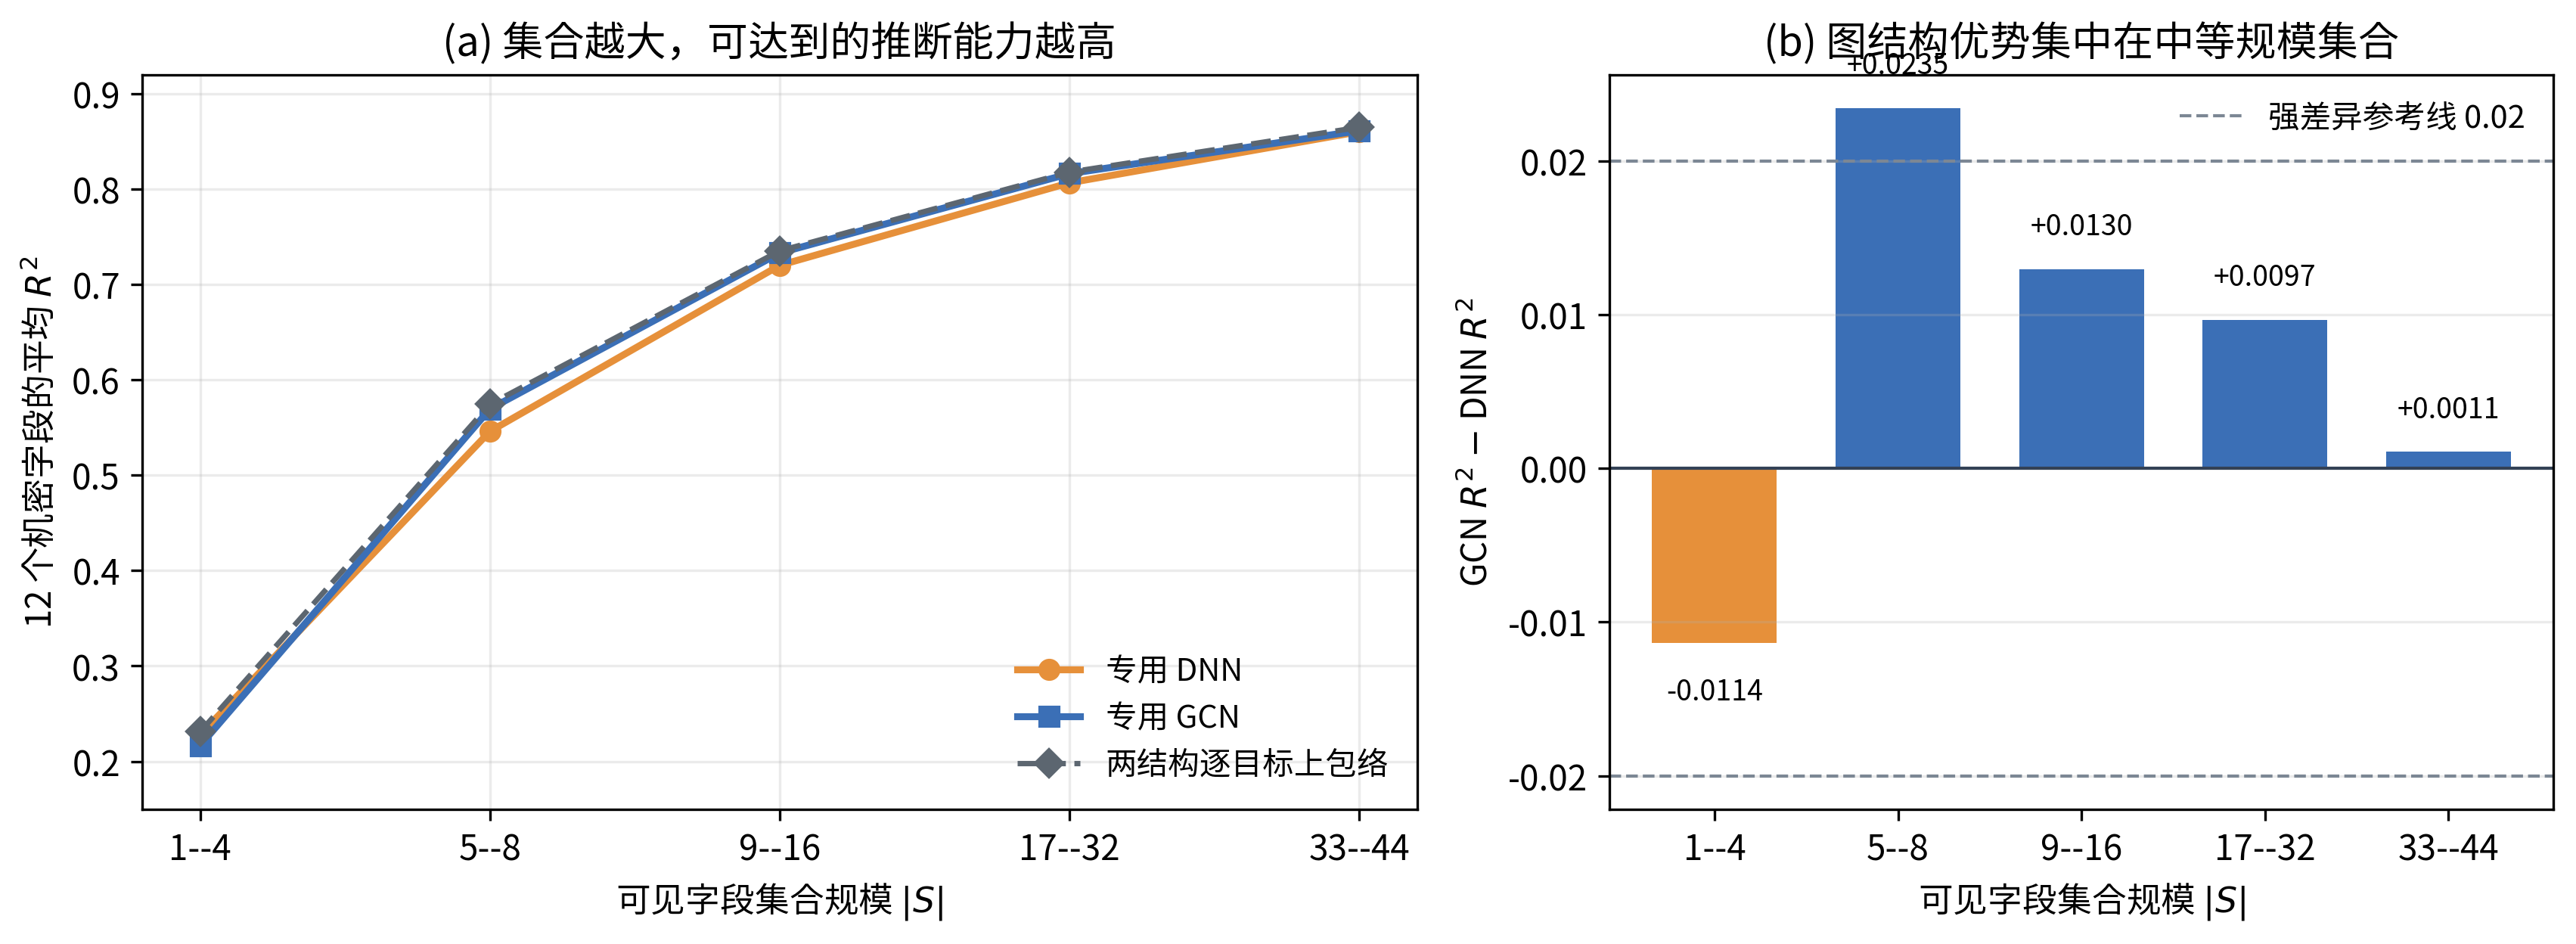
\includegraphics[width=0.98\textwidth]{attacker_scale.png}
  \caption{专用攻击者随可见集合规模的表现。左图显示集合规模效应；右图显示 GCN 相对 DNN 的增益。}
  \label{fig:attacker-scale}
\end{figure}

\begin{table}[H]
  \centering
  \caption{50 个宽尺寸随机集合上的专用攻击者比较}
  \label{tab:attacker}
  \begin{threeparttable}
  \begin{tabular}{@{}lrrrrr@{}}
    \toprule
    $|S|$ 区间 & 集合数 & DNN 平均 $\Rtwo$ & GCN 平均 $\Rtwo$
    & GCN$-$DNN & GCN 胜率\\
    \midrule
    1--4   & 10 & 0.2281 & 0.2167 & $-0.0114$ & 0.20\\
    5--8   & 10 & 0.5460 & \textbf{0.5695} & \textbf{+0.0235} & 0.70\\
    9--16  & 10 & 0.7200 & \textbf{0.7330} & \textbf{+0.0130} & 0.80\\
    17--32 & 10 & 0.8065 & \textbf{0.8162} & +0.0097 & 0.90\\
    33--44 & 10 & 0.8601 & 0.8612 & +0.0011 & 0.40\\
    \midrule
    全部   & 50 & 0.6321 & \textbf{0.6393} & +0.0072 & 0.60\\
    \bottomrule
  \end{tabular}
  \begin{tablenotes}\footnotesize
    \item “胜率”表示在同一集合上 GCN 的 12 目标平均 $\Rtwo$ 高于 DNN 的比例。差值超过 0.02 可视为强于两架构平均噪声底的参考量级。
  \end{tablenotes}
  \end{threeparttable}
\end{table}

图结构优势具有明确区间，而不是“规模越大，GCN 优势越大”。极小集合中可见边过少，GCN 无法充分聚合，DNN 反而高 0.0114；中等集合中既保留了可用的 general-general 关系，又远离完整输入，GCN 的邻居替代机制最有效；当接近完整输入时，两种模型都已达到较高 $\Rtwo$，增益趋于饱和。因此，\emph{推断能力本身随集合规模显著上升，而 GCN 相对 DNN 的小幅优势主要出现在 5--16 个字段的中等规模集合。}

\subsection{RQ2：任意集合 Oracle 的保真度}

图\ref{fig:oracle}和表\ref{tab:oracle}显示，当前通用 MLP-Oracle 在所有集合类型和相同步数下都比 GNN-Oracle 更接近专用 DNN 重训。以宽尺寸集合为例，$K=0$ 时逐目标 MAE 为 0.0767 对 0.1362；$K=200$ 后为 0.0194 对 0.0784。三个 Oracle 种子的复核保持同一结论，因此不能把专用 GCN 在中等规模集合上的优势外推为“通用 GNN-Oracle 更准确”。

\begin{figure}[H]
  \centering
  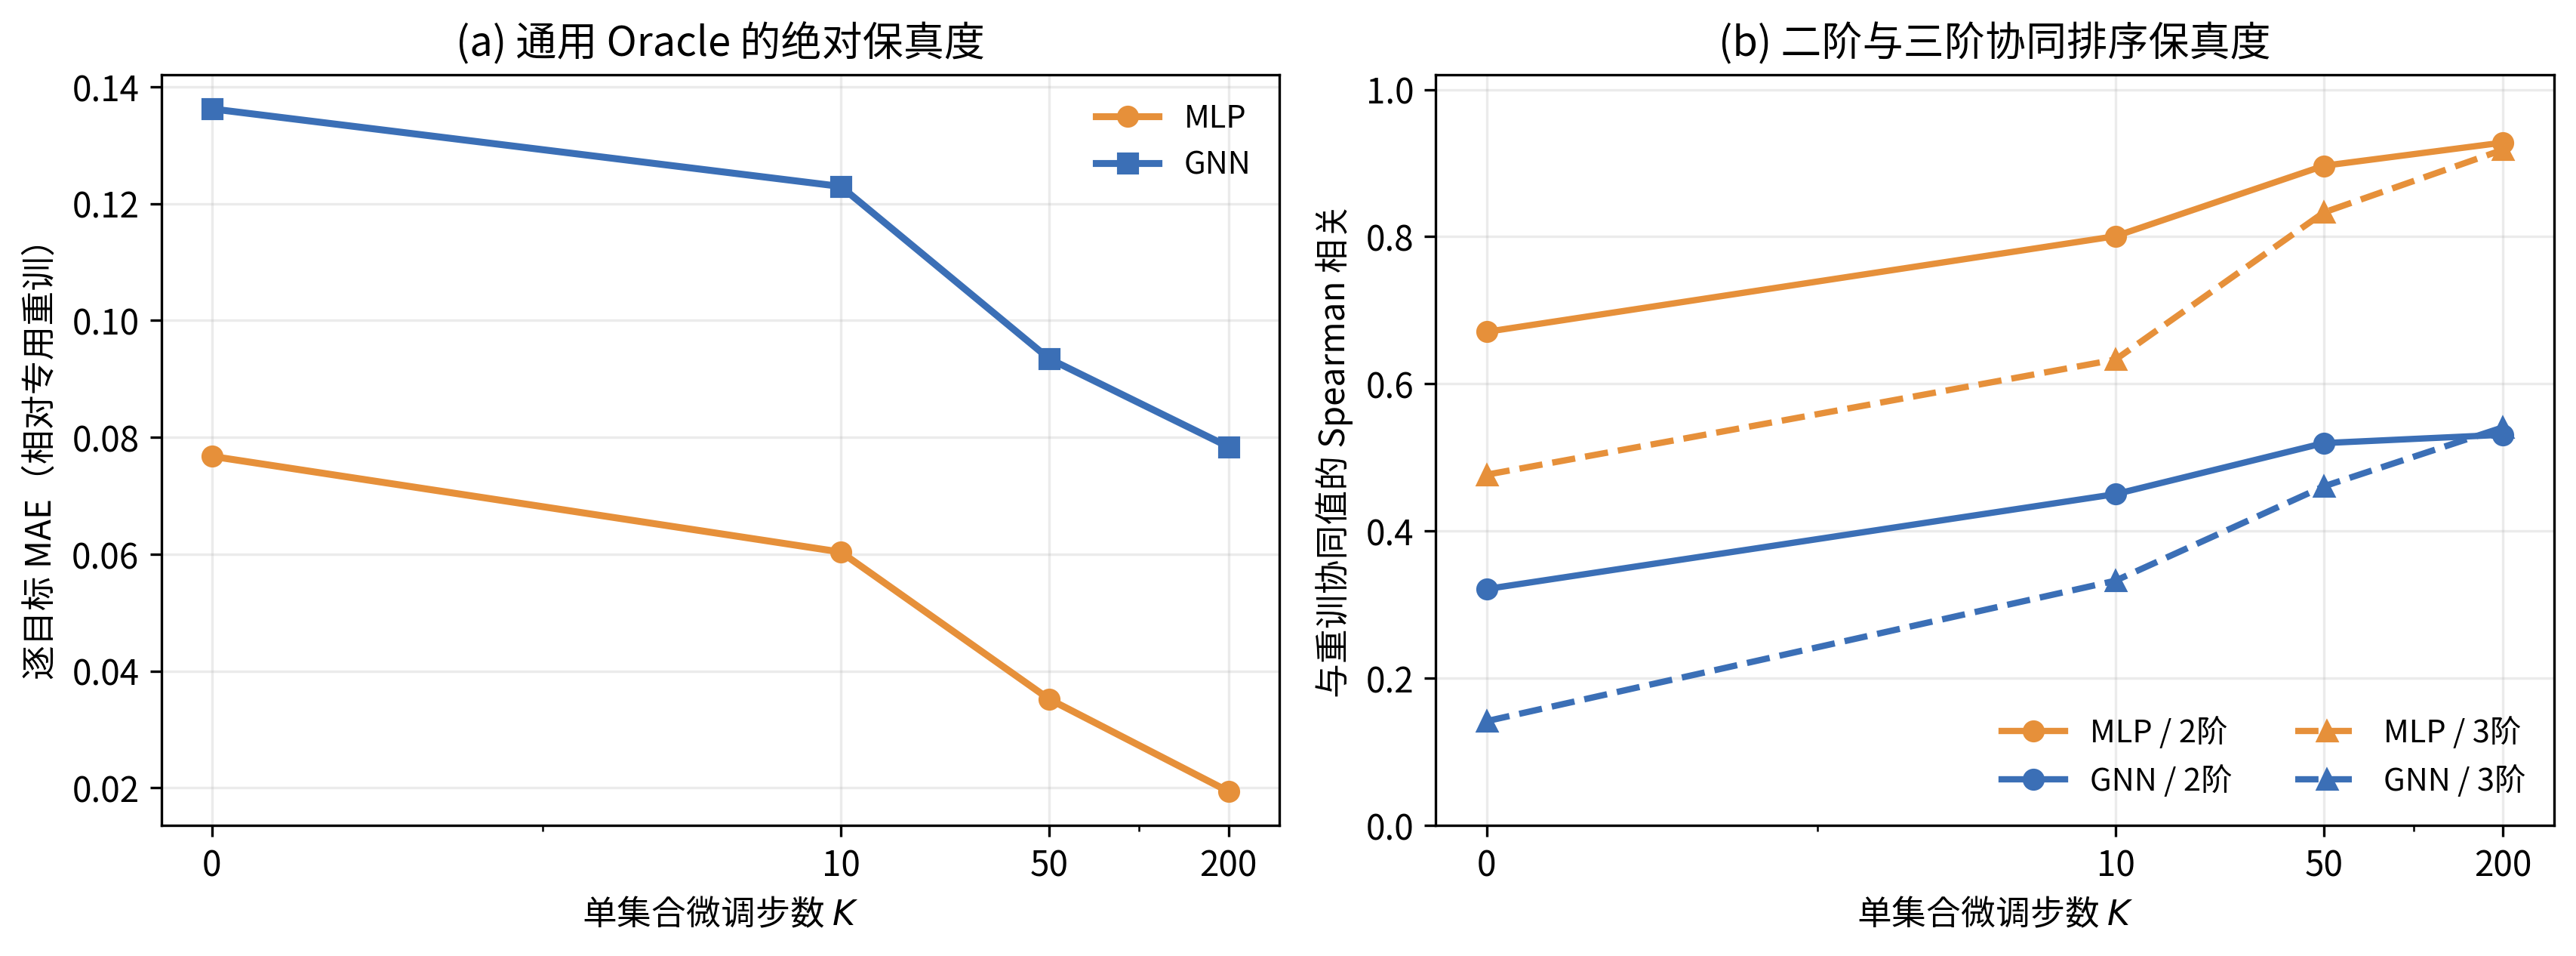
\includegraphics[width=0.98\textwidth]{oracle_fidelity.png}
  \caption{通用 MLP/GNN Oracle 的保真度。左：宽尺寸集合的绝对误差；右：二阶与三阶协同排序相对重训真值的一致性。}
  \label{fig:oracle}
\end{figure}

\begin{table}[H]
  \centering
  \caption{通用 Oracle 相对专用 DNN 重训的逐目标 MAE}
  \label{tab:oracle}
  \begin{tabular}{@{}llrrrr@{}}
    \toprule
    集合类型 & 架构 & $K=0$ MAE & $K=200$ MAE & $K=200$ 秒/集合 & 误差降幅\\
    \midrule
    \multirow{2}{*}{宽尺寸集合}
      & MLP & 0.0767 & \textbf{0.0194} & 0.392 & 74.7\%\\
      & GNN & 0.1362 & 0.0784 & 3.076 & 42.4\%\\
    \midrule
    \multirow{2}{*}{字段对}
      & MLP & 0.0495 & \textbf{0.0150} & 0.402 & 69.7\%\\
      & GNN & 0.0813 & 0.0350 & 3.104 & 57.0\%\\
    \midrule
    \multirow{2}{*}{三元组}
      & MLP & 0.0912 & \textbf{0.0213} & 0.394 & 76.6\%\\
      & GNN & 0.1381 & 0.0436 & 3.109 & 68.4\%\\
    \bottomrule
  \end{tabular}
\end{table}

原因在于两个任务的归纳偏置不同。专用 GCN 只需优化一个 $S$，结构先验能够帮助沿相关边重组信息；通用 GNN-Oracle 必须用同一组消息传递参数拟合大量不同诱导子图，静态相关图和注意力瓶颈造成系统性低估。MLP 虽不显式使用图，但其宽隐藏层更容易拟合从 $[\bm x\odot\bm m,\bm m]$ 到多目标条件期望的复杂映射。

据此，本文使用专用 GCN 增强攻击上限审计，使用保真度更高的 MLP-Oracle 扫描集合空间。对二阶协同，MLP-Oracle 从 $K=0$ 的 Spearman 0.6708 提升到 $K=200$ 的 0.9279；扩展到 $K=500$ 后达到 0.9597，top-20 重合率 0.95，单集合耗时 1.008 s。相比每个集合约数分钟的从头重训，该方案把 946 个字段对的高保真计算压缩到分钟量级。

\subsection{RQ3a：二阶协同图}

对 44 个字段的全部 946 个无序对逐目标计算式\eqref{eq:pair}。图\ref{fig:synergy-graph}展示最大目标协同权重最高的一组可解释子图。粗边集中在同一燃料的“发电功率--发电占比”字段对，说明协同图捕捉到了稳定的物理关系，而不是随机相关。

\begin{figure}[H]
  \centering
  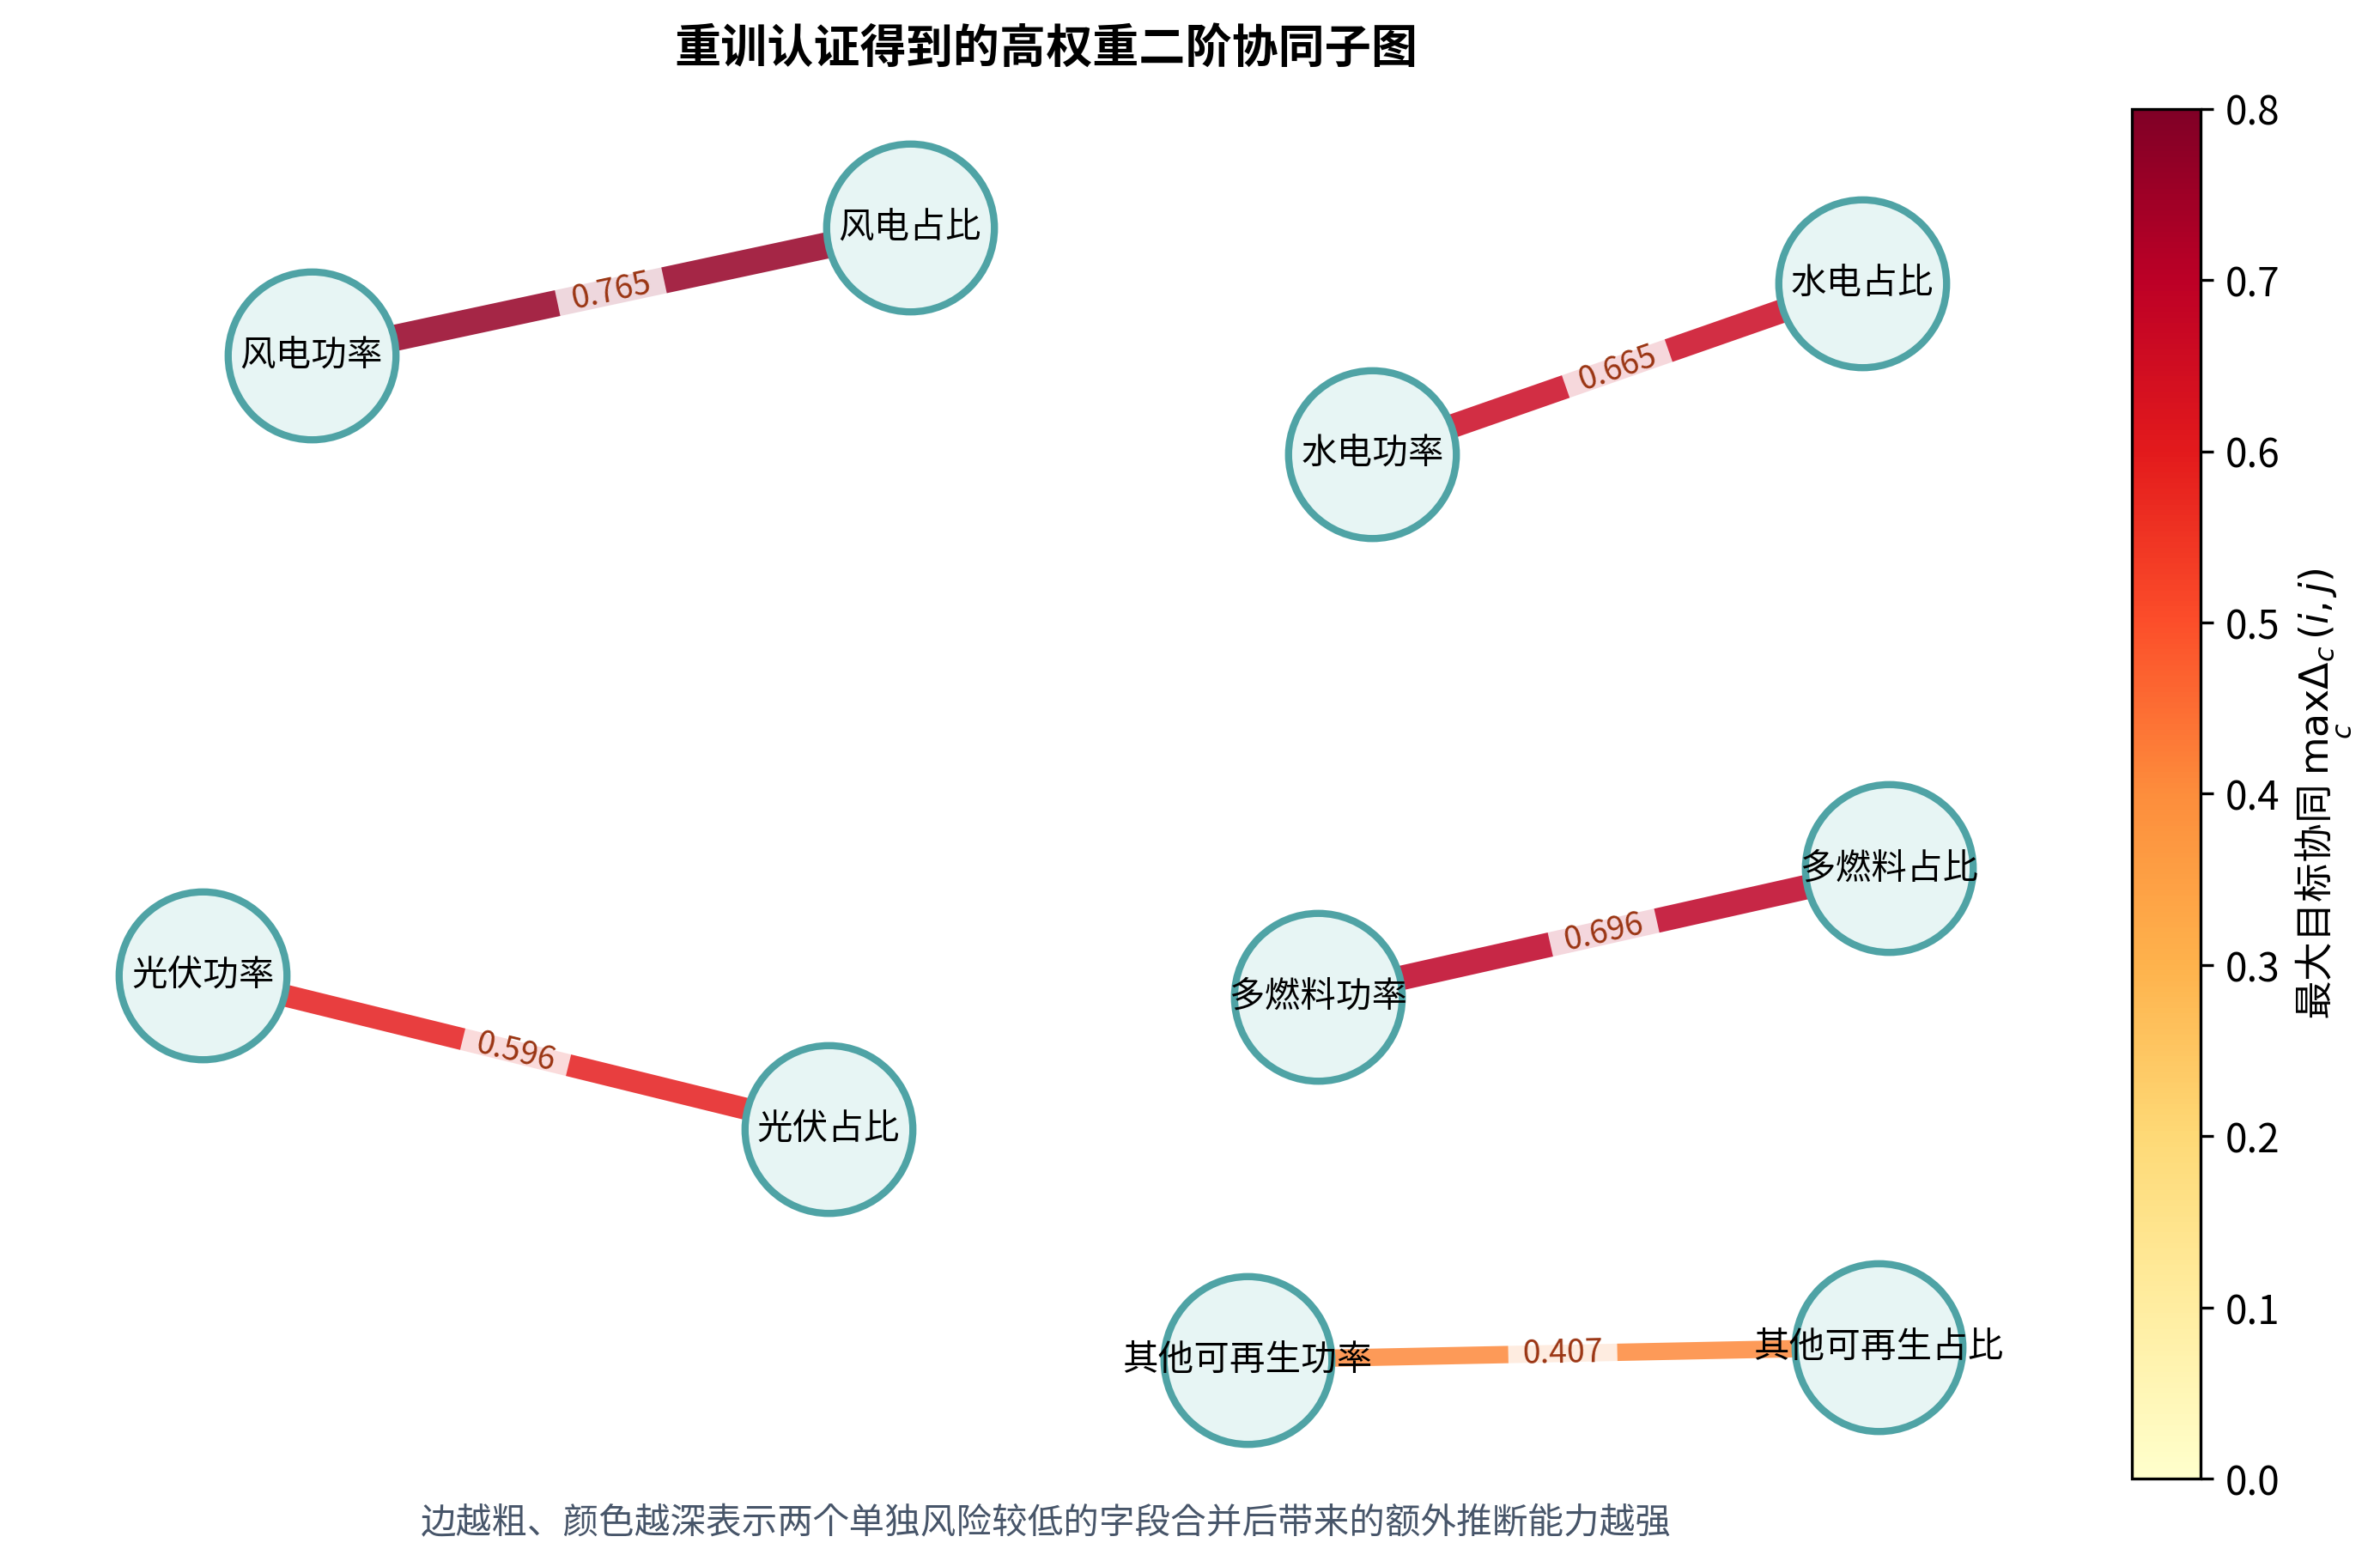
\includegraphics[width=0.82\textwidth]{synergy_graph.png}
  \caption{重训认证得到的高权重二阶协同子图。边权为 12 个机密目标中的最大 $\Delta_c(i,j)$。}
  \label{fig:synergy-graph}
\end{figure}

表\ref{tab:pair-synergy}给出强协同案例。风电功率单独推断总发电量的 $\Rtwo$ 仅为 0.0638，风电占比单独为 0.1623，但二者合并后达到 0.9277，增量协同为 0.7654。光伏功率单独几乎无预测力（0.0057），与光伏占比合并后却达到 0.6954。这正是单字段敏感度最容易漏掉的“单看安全、合体泄露”。

\begin{table}[H]
  \centering
  \caption{重训认证的代表性二阶协同}
  \label{tab:pair-synergy}
  \begin{tabularx}{\textwidth}{@{}llYrrrr@{}}
    \toprule
    字段 $i$ & 字段 $j$ & 机密目标 $c$
    & $v_c(i)$ & $v_c(j)$ & $v_c(ij)$ & $\Delta_c(i,j)$\\
    \midrule
    风电功率 & 风电占比 & 总发电量
      & 0.0638 & 0.1623 & 0.9277 & \textbf{0.7654}\\
    风电功率 & 风电占比 & 计量负荷
      & 0.0586 & 0.1527 & 0.9033 & 0.7506\\
    多燃料功率 & 多燃料占比 & 总发电量
      & 0.2010 & 0.0779 & 0.8967 & 0.6957\\
    水电功率 & 水电占比 & 总发电量
      & 0.2921 & 0.1346 & 0.9572 & 0.6651\\
    光伏功率 & 光伏占比 & 总发电量
      & 0.0057 & 0.0992 & 0.6954 & 0.5962\\
    \bottomrule
  \end{tabularx}
\end{table}

\subsection{RQ3b：三阶不可约协同}

二阶协同仍不能描述“发电侧两个字段加负荷侧一个字段”共同决定交换功率的关系。本文用 $K=200$ 的 MLP-Oracle 扫描全部 $\binom{44}{3}=13244$ 个三元组，再重训 197 个高分候选和 200 个随机三元组。每个三元组对 12 个机密目标产生一条三阶增量记录。

如图\ref{fig:triple}所示，候选组中有 314/2364 条逐目标记录满足 $\Delta_c^{(3)}>0.1$，随机组只有 19/2400 条；候选组最大值为 0.4547。对具有扫描估计和重训结果的记录，Spearman 为 0.800，说明 Oracle 适合排序筛选，但最终幅值仍应由重训认证。

\begin{figure}[H]
  \centering
  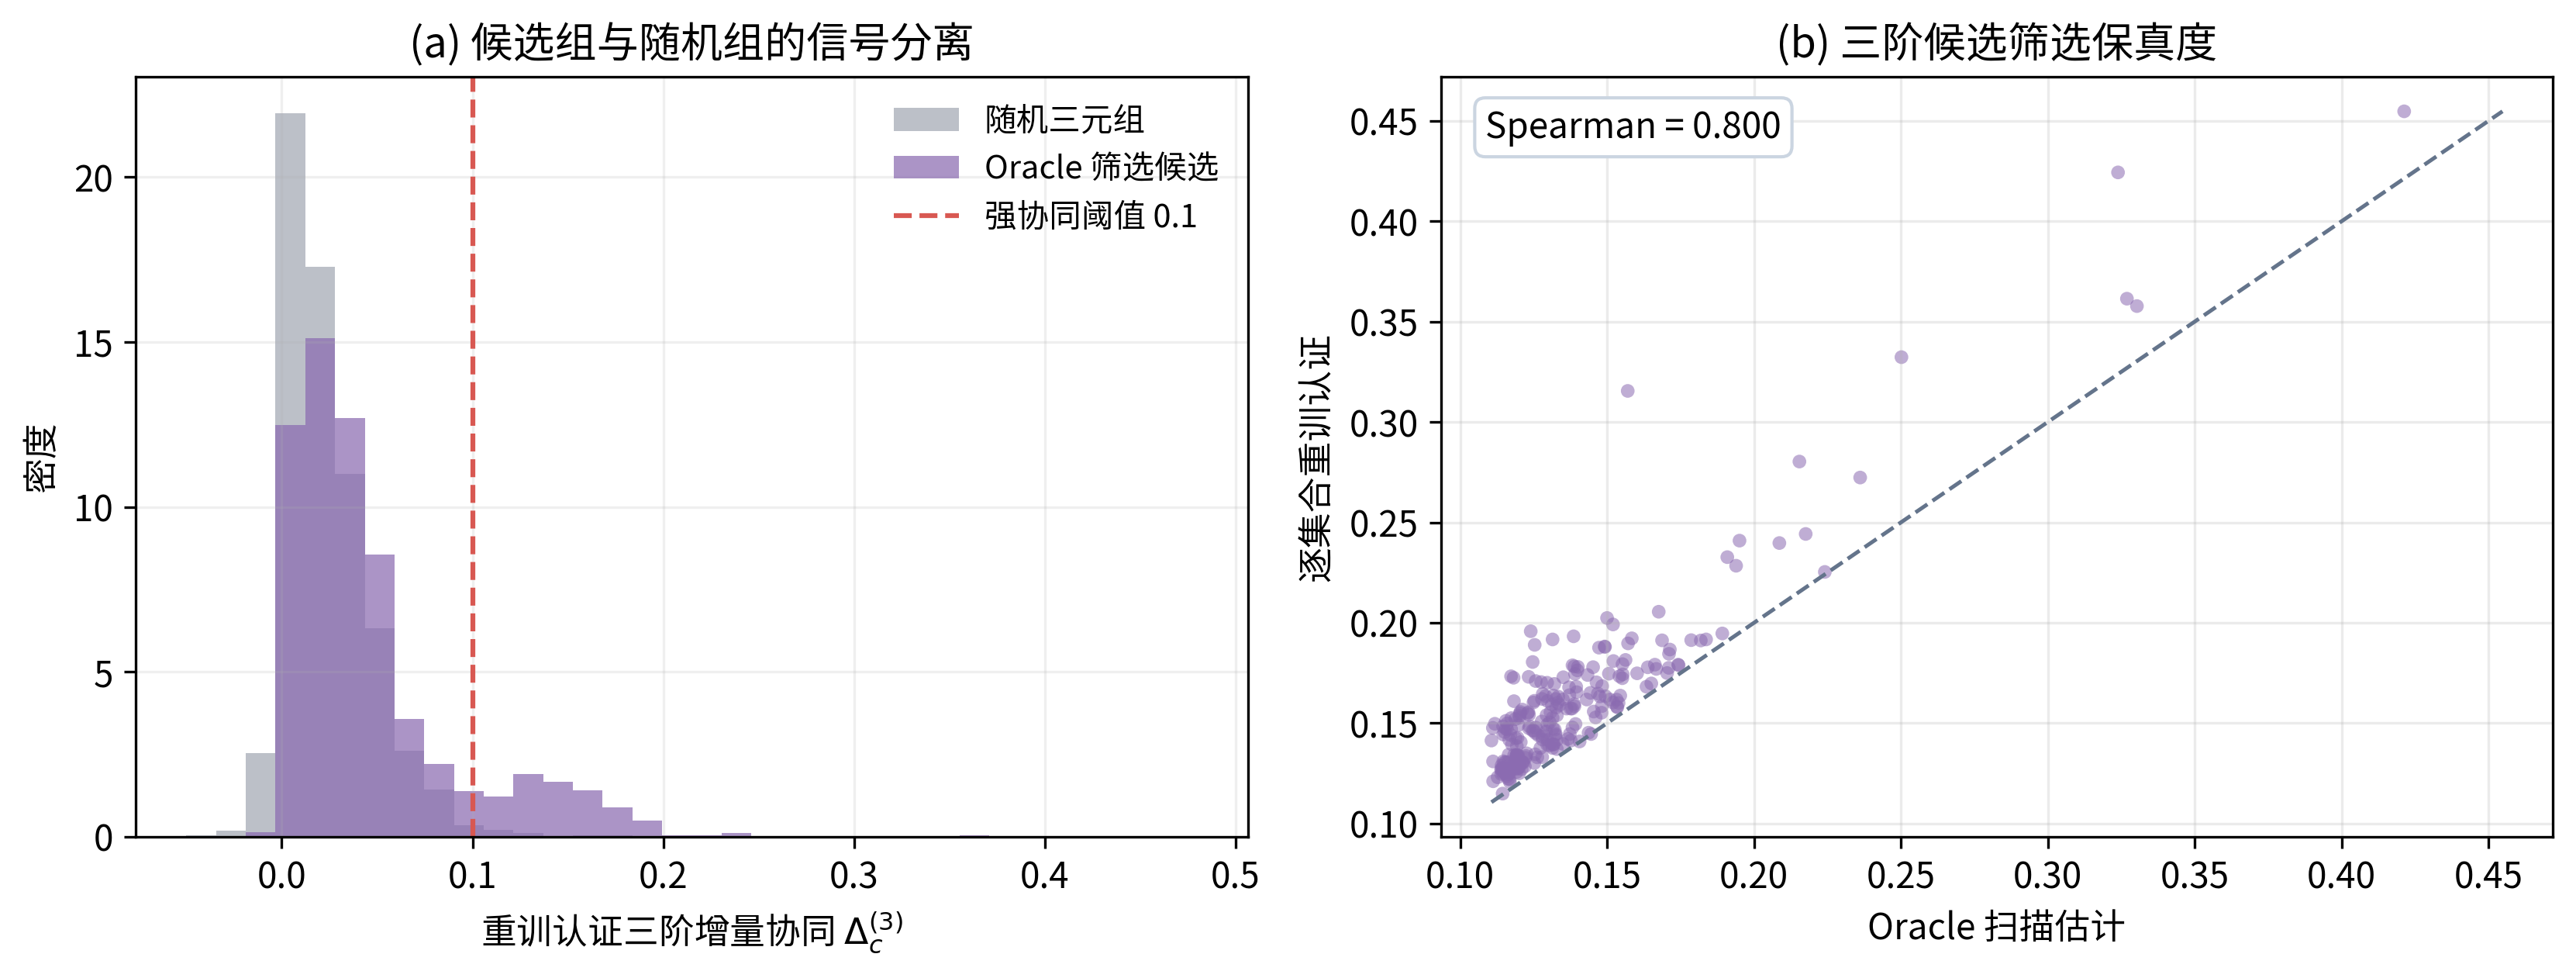
\includegraphics[width=0.98\textwidth]{triple_certification.png}
  \caption{三阶协同筛选与重训认证。候选组的右尾明显强于随机组；Oracle 估计与重训真值保持较高排序一致性。}
  \label{fig:triple}
\end{figure}

最强案例是“燃气发电功率 + 燃气发电占比 + 最新负荷预测”推断净实际交换功率。三元组 $\Rtwo$ 为 0.6930，最好二元子集只有 0.2383，因此 $\Delta^{(3)}=0.4547$。其物理解释为：燃气功率与占比共同提供总发电量线索，负荷预测提供负荷侧线索，而净交换近似由发电与负荷差决定。只缺任一类信息时都不能完整恢复目标，故该结构是不可约三方超边，而不是两两强边的简单重复。

\subsection{RQ4：噪声底与近似边界}

\textbf{训练噪声底。} 对同一集合、同一切分仅改变训练随机种子，专用 DNN 的 12 目标平均 $\Rtwo$ 标准差中位数为 0.0015、最大值为 0.0023；GCN 分别为 0.0039 和 0.0114。因而中等规模集合上 0.0235 的 GCN 增益超过平均噪声量级，而 33--44 区间的 0.0011 不能解释为实质优势。

\textbf{零填充伪影。} 将完整输入模型的缺失字段直接置零，得到的二阶协同与逐集合重训真值 Spearman 仅为 0.351；平均协同为 0.012，而重训为 0.041，低估约 3.4 倍。这验证了随机掩码训练和重训认证的必要性。

\textbf{协同比直接敏感度更难。} $v_c(ij)$、$v_c(i)$ 和 $v_c(j)$ 的估计误差会在式\eqref{eq:pair}中相减叠加。通用 MLP-Oracle 对直接集合值的排序在宽尺寸集合上接近 0.99，但 $K=0$ 的二阶协同排序只有 0.67。只有微调闭合各集合的系统偏差后，协同排序才提升到 0.96。因此，不能用“直接敏感度排序很好”替代协同保真度验证。

\section{讨论}

\subsection{图结构的有效区间与模型分工}

集合规模实验表明，关系归纳偏置的收益取决于任务粒度。对固定集合分别训练专用攻击者时，GCN 在 5--16 个字段的区间取得最稳定的增益：此时诱导子图仍保留足够多的有效边，消息传递可以在缺失直接字段时利用邻域关系补全推断路径；在极小集合上，可见边过少使图聚合难以发挥作用，而在接近全字段输入时，两类模型均趋于饱和。由此可见，集合规模增大首先提升的是总体可推断性，图结构带来的额外收益则集中于关系信息最有价值的中等规模区间。

通用 Oracle 的任务不同：同一组参数需要覆盖大量掩码及其对应的条件分布。当前实验中，MLP-Oracle 的逐点保真度优于 GNN-Oracle，而专用 GCN 仍能提高部分集合的攻击上限。两组结果共同支持按功能组织模型：字段图用于表达关系并增强专用攻击审计，随机掩码 Oracle 用于大规模候选排序，最终风险值由逐集合重训认证。该分工使图结构的作用落在其有效区间，同时保持集合扫描的精度与效率。

\subsection{协同图与高阶泄露结构}

二阶协同边高度集中在“燃料出力--燃料占比”字段对，三阶超边则进一步把发电侧关系与负荷侧信息连接起来。这种从强边到不可约超边的扩展说明，组合泄露并非若干高敏感字段的简单叠加，而是由完整物理约束被逐步补全所产生。尤其是单字段推断能力接近零的字段仍可能参与高权重协同边，因而仅依据节点分数排序或静态相关系数删减字段，无法覆盖主要泄露路径。

协同图还为数据发布控制提供了直接的图论接口。若将超过阈值的二阶边和三阶超边视为必须被阻断的风险关系，则“最少隐藏哪些字段”可表示为加权顶点覆盖或超图击中集问题；边权可进一步结合机密目标的重要度与重训置信度。这样，集合敏感度 Oracle 负责给出可靠的组合风险，图优化则把风险评估转化为可执行的字段保护方案。

\subsection{跨系统扩展的结构基础}

输入维度固定的 MLP 与 44 个字段位置直接绑定，而图模型通过共享消息函数和邻域聚合编码关系\citep{battaglia2018relational,hamilton2017graphsage}。当另一电力系统能够把字段映射为统一类型，并按相同统计准则重建字段图时，消息传递参数无需依赖原系统的节点顺序，因而更适合采用“重建图结构、复用聚合器、少量微调目标头”的迁移方式。随着字段规模扩大，组合数按 $2^n$ 增长，而扫描—认证流程只对高分候选投入重训预算，也为更大字段图提供了可扩展的计算路径。

本文实证结果对应 PJM 数据上的同分布推断场景，经验攻击上限由现有 DNN/GCN 模型族近似；跨区域迁移与时间外推属于不同的泛化问题。后续可在统一字段类型编码下分别比较零样本、少样本和全量训练性能，从而检验上述结构迁移机制。

\section{结论}

本文针对单字段敏感度无法表达组合泄露的问题，提出面向任意字段集合的图结构敏感度评估方法：以字段推断图组织关系，以集合函数 $v_c(S)$ 定义攻击者在任意可见集合上的推断能力，并通过随机掩码 Oracle、微调与重训认证实现大规模组合空间的可靠查询。实验表明，推断能力随可见集合规模显著增强，专用 GCN 在中等规模集合上取得稳定增益；由同一集合函数构建的二阶协同图和三阶协同超图进一步识别出具有明确物理机制的组合泄露路径。该方法将任意集合风险评估、图结构推断与高阶协同发现统一起来，为电力数据的分级共享和字段组合防护提供了图论化分析基础。

\begin{thebibliography}{99}
\small

\bibitem{fredrikson2015model}
FREDRIKSON M, JHA S, RISTENPART T.
Model inversion attacks that exploit confidence information and basic countermeasures[C]//
Proceedings of the 22nd ACM SIGSAC Conference on Computer and Communications Security.
New York: ACM, 2015: 1322--1333.

\bibitem{mehnaz2022sensitive}
MEHNAZ S, DIBBO S V, KABIR E, et al.
Are your sensitive attributes private? Novel model inversion attribute inference attacks on classification models[C]//
31st USENIX Security Symposium.
Berkeley: USENIX Association, 2022: 4579--4596.

\bibitem{hu2026ignn}
HU B, NIE R, ZHOU Y, et al.
IGNN: An inference graph neural network for data sensitivity assessment considering data inference leakage in cyber-physical power grid[J].
IEEE Transactions on Smart Grid, 2026, Early Access.
DOI: 10.1109/TSG.2026.3667966.

\bibitem{kipf2017gcn}
KIPF T N, WELLING M.
Semi-supervised classification with graph convolutional networks[C]//
International Conference on Learning Representations.
2017.

\bibitem{velickovic2018gat}
VELI\v{C}KOVI\'C P, CUCURULL G, CASANOVA A, et al.
Graph attention networks[C]//
International Conference on Learning Representations.
2018.

\bibitem{jethani2022fastshap}
JETHANI N, SUDARSHAN M, COVERT I C, et al.
FastSHAP: Real-time Shapley value estimation[C]//
International Conference on Learning Representations.
2022.

\bibitem{shapley1953value}
SHAPLEY L S.
A value for $n$-person games[M]//
KUHN H W, TUCKER A W, eds.
Contributions to the Theory of Games II.
Princeton: Princeton University Press, 1953: 307--317.

\bibitem{harsanyi1963bargaining}
HARSANYI J C.
A simplified bargaining model for the $n$-person cooperative game[J].
International Economic Review, 1963, 4(2): 194--220.

\bibitem{grabisch1999interaction}
GRABISCH M, ROUBENS M.
An axiomatic approach to the concept of interaction among players in cooperative games[J].
International Journal of Game Theory, 1999, 28(4): 547--565.

\bibitem{pjmdataminer}
PJM INTERCONNECTION.
Data Miner 2[EB/OL].
\url{https://www.pjm.com/markets-and-operations/etools/data-miner-2},
2026-07-18.

\bibitem{battaglia2018relational}
BATTAGLIA P W, HAMRICK J B, BAPST V, et al.
Relational inductive biases, deep learning, and graph networks[J].
arXiv preprint arXiv:1806.01261, 2018.

\bibitem{hamilton2017graphsage}
HAMILTON W L, YING R, LESKOVEC J.
Inductive representation learning on large graphs[C]//
Advances in Neural Information Processing Systems.
2017, 30.

\bibitem{lundberg2017shap}
LUNDBERG S M, LEE S I.
A unified approach to interpreting model predictions[C]//
Advances in Neural Information Processing Systems.
2017, 30.

\bibitem{berge1989hypergraphs}
BERGE C.
Hypergraphs: Combinatorics of Finite Sets[M].
Amsterdam: North-Holland, 1989.

\end{thebibliography}


\end{document}
